\tikzset{>=latex} % for LaTeX arrow head
\colorlet{Ecol}{orange!90!black}
\colorlet{EcolFL}{orange!90!black}
\colorlet{veccol}{green!45!black}
\colorlet{Bcol}{violet!90}
\colorlet{Bcol1}{violet!80!blue!90}
\colorlet{Bcol2}{violet!80!red!90}
\colorlet{BFcol}{red!60!black}
\colorlet{veccol}{green!45!black}
\colorlet{Icol}{blue!70!black}
\tikzstyle{BField}=[->,thick,Bcol]
\tikzstyle{current}=[->,Icol,thick]
\tikzstyle{force}=[->,thick,BFcol]
\tikzstyle{vector}=[->,thick,veccol]
\colorlet{pluscol}{red!60!black}
\colorlet{minuscol}{blue!60!black}
\tikzstyle{charge+}=[very thin,draw=black,top color=red!50,bottom color=red!90!black,shading angle=20,circle,inner sep=0.3]
\tikzstyle{charge-}=[very thin,draw=black,top color=blue!50,bottom color=blue!80,shading angle=20,circle,inner sep=0.3]
\tikzstyle{metal}=[top color=black!15,bottom color=black!25,middle color=black!20,shading angle=10]
\tikzstyle{light metal}=[top color=black!10,bottom color=black!15,middle color=black!6,shading angle=10]
\tikzset{
  EFieldLine/.style={thick,EcolFL,decoration={markings,mark=at position #1 with {\arrow{latex}}},
                     postaction={decorate}},
  EFieldLine/.default=0.5,
  BFieldLine/.style={thick,Bcol,decoration={markings,mark=at position #1 with {\arrow{latex}}},
                                 postaction={decorate}},
  BFieldLine/.default=0.5,
  pics/Bin/.style={
    code={
      \def\R{0.12}
      \draw[pic actions,line width=0.6,#1,fill=white] % ,thick
        (0,0) circle (\R) (-135:.75*\R) -- (45:.75*\R) (-45:.75*\R) -- (135:.75*\R);
  }},
  pics/Bout/.style={
    code={
      \def\R{0.12}
      \draw[pic actions,line width=0.6,#1,fill=white] (0,0) circle (\R);
      \fill[pic actions,#1] (0,0) circle (0.3*\R);
  }},
  pics/Bin/.default=Bcol,
  pics/Bout/.default=Bcol,
  pics/magnet/.style={ %args={#1}
    code={
      \def\h{0.9}
      \coordinate (-N) at (0,\h);
      \coordinate (-S) at (0,-\h);
      \draw[pic actions,thick,top color=red!60,bottom color=red!90,shading angle=20]
        (-0.8*\h/2,0) rectangle ++(0.8*\h,\h);
      \draw[pic actions,thick,top color=blue!60,bottom color=blue!90,shading angle=20]
        (-0.8*\h/2,0) rectangle ++(0.8*\h,-\h);
      \node[pic actions] at (0, \h/2) {\textbf{N}};
      \node[pic actions] at (0,-\h/2) {\textbf{S}};
  }},
}
\tikzstyle{measure}=[<->,fill=white,midway,outer sep=0]
\contourlength{1.5pt}

% FLUX-CHANGING LOOP




% MOVING CONDUCTOR


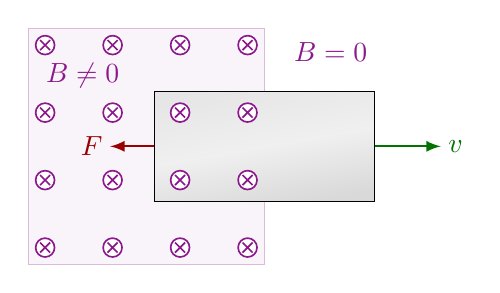
\begin{tikzpicture}
  \def\NBx{4}
  \def\NBy{4}
  \def\WB{3}
  \def\NQ{5}
  \def\L{2.8}
  \def\W{1.4}
  
  % MAGNETIC FIELDLINES
  \draw[Bcol!30,fill=Bcol!5] (-\WB,-\WB/2) rectangle++ (\WB,\WB);
  
  % CONDUCTOR
  \draw[light metal] (-\L/2,-\W/2) rectangle++ (\L,\W);
  \draw[vector] (\W,0) --++ (0.6*\W,0) node[right=-1] {$\vb{v}$};
  \draw[force] (-\W,0) --++ (-0.4*\W,0) node[left=-1] {$\vb{F}$};
  %\draw[EFieldLine=0.55] ( 0.29*\W,0.9*\L) --++ (0,-0.8*\L);
  
  % MAGNETIC FIELDLINES
  \foreach \i [evaluate={\y=-\WB/2+(\i-0.75)*\WB/(\NBy-0.5)}] in {1,...,\NBy}{
    \foreach \j [evaluate={\x=-\WB+(\j-0.75)*\WB/(\NBx-0.5)}] in {1,...,\NBx}{
      \pic[scale=1] at (\x,\y) {Bin};
    }
  }
  \node[Bcol] at (-0.77*\WB,0.30*\WB) {$\vb{B}\neq0$};
  \node[Bcol] at ( 0.28*\WB,0.40*\WB) {$\vb{B}=0$};
  
\end{tikzpicture}
